%!TEX root = lec06_transactions.tex

%%%%%%%%%%%%%%%%%%%%%%%%%% ----- Transactions are programs
%
% -------------------------------------
%
\begin{frame}[fragile]{Transactions inside programs}

Transactions can be as simple as a command issued from the command line interface of the DBMS, or as complex as a series of SQL statements mixed with arbitrary computations by a program.


\begin{lstlisting}[style=C]
...
char *stmt = "UPDATE R SET a=? where id=?;";
sqlite3_prepare_v2(db, stmt, -1, &stmt_q, 0);

sqlite3_exec(db, "BEGIN TRANSACTION;", NULL, NULL, NULL);
  x = f(...); //compute some value x
  _id = input(...); //ask user for input 
  sqlite3_bind_int64(stmt_q, 1, (sqlite3_int64), x);
  sqlite3_bind_int64(stmt_q, 2, (sqlite3_int64), _id);
  if (rc = sqlite3_step(stmt_q)) != SQLITE_ROW) ...
  ...
  //another query or update can go here...
sqlite3_exec(db, "COMMIT;", NULL, NULL, NULL);
...
\end{lstlisting}
\end{frame}

\begin{frame}

\vskip2em

\begin{columns}[onlytextwidth]
\begin{column}{0.6\textwidth}
Every operation of the transaction that needs to read or write data inside the DBMS is monitored and logged, to ensure the correct execution of the transaction.
\vskip0.75em

The DBMS must also schedule the execution of such requests to optimize performance.
\end{column}

\begin{column}{0.4\textwidth}
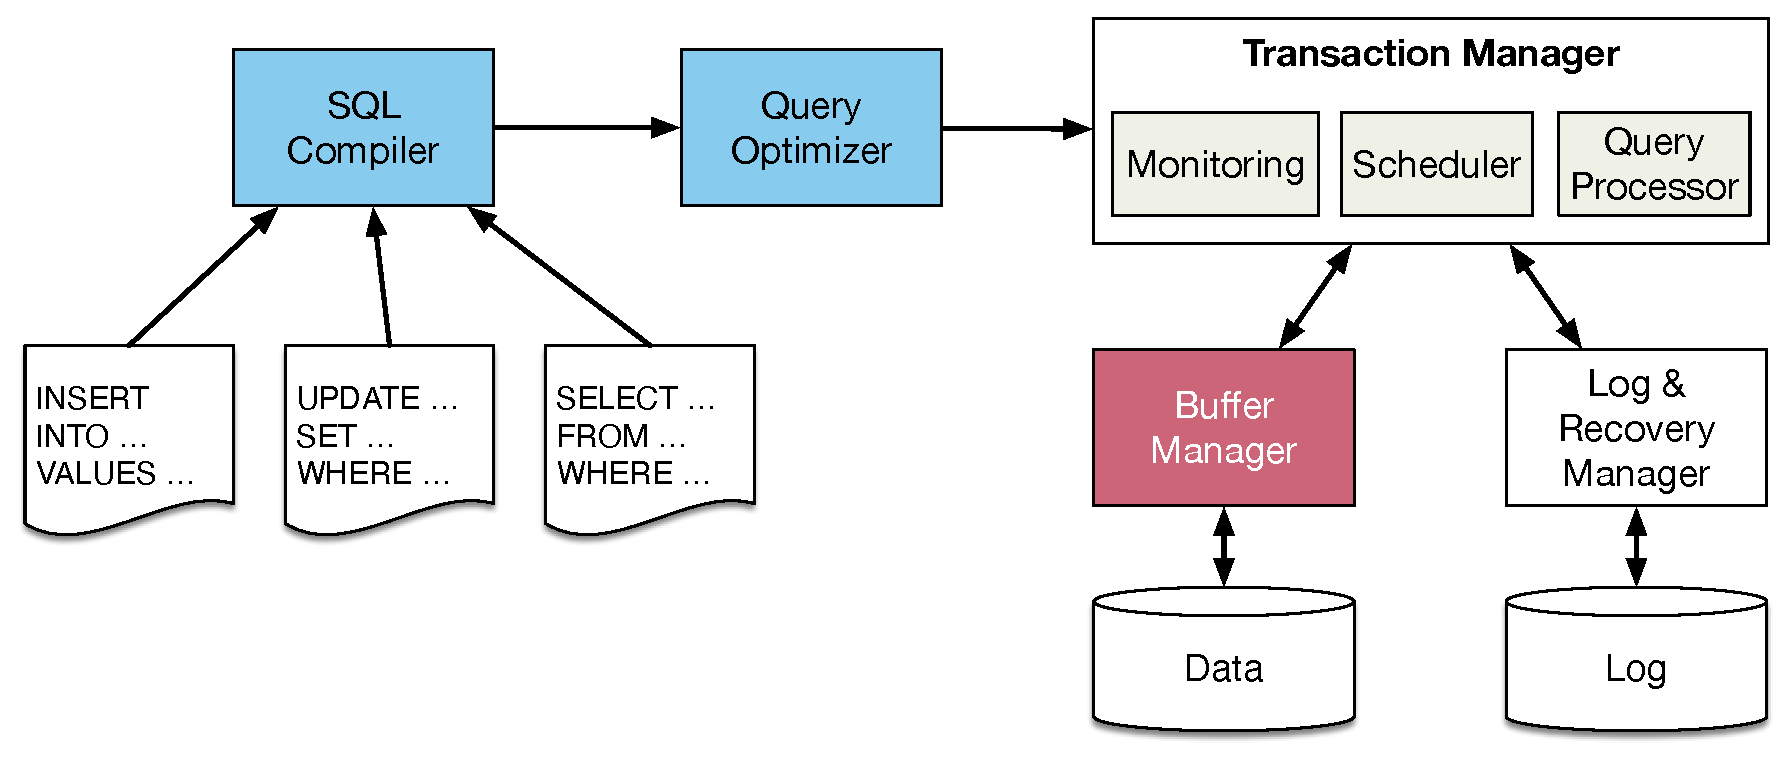
\includegraphics[trim=515 0 0 0,clip,width=0.9\textwidth]{../lec00_intro/figures/dbms_architecture.eps}
\end{column}

\end{columns}

\vskip0.5em

Keep in mind that many transactions can execute concurrently, and the DBMS needs to manage all of them simultaneously.

\end{frame}
	

%
% -------------------------------------
%


\begin{frame}[fragile]{Running example}

Consider this oversimplified banking situation:

\vskip1em

\begin{columns}
\begin{column}{0.2\textwidth}
\scalebox{0.8}{\usebox{\exampleA}}
\end{column}
\begin{column}{0.3\textwidth}
\scalebox{0.8}{\usebox{\exampleB}}
\end{column}
\end{columns}

\vskip2em

\begin{columns}[onlytextwidth]
\begin{column}{0.4\textwidth}
And assume Nuttah requests to transfer money from her\\ checking account into\\ her investments.
\end{column}
\begin{column}{0.6\textwidth}
\scalebox{0.75}{\usebox\UPDATEexample}
\end{column}
\end{columns}

\vskip2em

Doing the transaction \textbf{atomically} prevents her losing money!
\end{frame}


%
% -------------------------------------
%
\begin{frame}[fragile]
\vskip1em

The attributes modified by the transaction are called the \textbf{\alert{database elements}} of the transaction. In some texts, these are defined as entire tuples.

\vskip2em

\begin{columns}[onlytextwidth]
\begin{column}{0.5\textwidth}
\scalebox{0.8}{\usebox{\exampleA}}
\end{column}
\begin{column}{0.5\textwidth}
\scalebox{0.8}{\usebox{\exampleB}}
\end{column}
\end{columns}

\vskip2em

These are the database elements that need to be modified by our example transaction:
\begin{itemize}[-,noitemsep,topsep=-0.5em]
\item The \lstinline[style=cmput391]{balance} attribute on tuple (with id) $t_1$.
\item The \lstinline[style=cmput391]{balance} attribute on tuple (with id) $t_2$.
\end{itemize}
\end{frame}

%
% -------------------------------------
%
\begin{frame}{Database elements, buffers, I/O, ...}

Recall the transfer unit for I/O operations in the DBMS are \emph{disk blocks}. Thus, before a database element can be modified, the block containing it must be retrieved from disk.

\textbf{DBMS I/O primitives}:

\begin{itemize}[-,noitemsep]
\item \INPUT{X}: copies the disk block containing element \texttt{X} to a memory buffer
\item \OUTPUT{X}: copies the memory buffer with element \texttt{X} to disk
\item \READ{X}{v}: copies the value of element \texttt{X} from the memory buffer into local variable \texttt{v} in the transaction program
\item \WRITE{X}{v}: copies the value of variable \texttt{v} in the local address space of the transaction to element \texttt{X} in the memory buffer
\end{itemize}

A call to either \READ{X}{v} or \WRITE{X}{v} calls \INPUT{X} if the database element \texttt{X} isn't already in memory.

\end{frame}


\newsavebox\compilerAddedCodeForConsistency
\savebox{\compilerAddedCodeForConsistency}{%
\begin{minipage}{0.4\textwidth}\footnotesize
\lstinline[style=SQL]{BEGIN TRANSACTION};\\
\texttt{A} $\leadsto t_1.\mathtt{balance}$;\\
\texttt{B} $\leadsto t_2.\mathtt{balance}$; \\
\READ{A}{v};\\
\ASSIGN{v}{v - 20};\\
\WRITE{A}{v};\\ 
\READ{B}{v};\\
\ASSIGN{v}{v + 20};\\
\WRITE{B}{v};\\
\OUTPUT{A};\\
\OUTPUT{B};\\
\COMMIT;
\end{minipage}}

%
% -------------------------------------
%
\begin{frame}[fragile]


\begin{columns}
\begin{column}{0.2\textwidth}
\scalebox{0.7}{\usebox{\exampleA}}
\end{column}
\begin{column}{0.375\textwidth}
\scalebox{0.7}{\usebox{\exampleB}}
\end{column}
\end{columns}

\vskip3em

\begin{columns}[onlytextwidth]
\begin{column}{0.5\textwidth}
Focusing only on the I/O and data modification operations, the transaction is abstracted as the following ``program'' that will be executed by the DBMS. 
\\[1em]
Here we are using the $\leadsto$ symbol to abstract the ``query'' part of the update statement that finds the tuple with the corresponding id. 
\end{column}
\begin{column}{0.4\textwidth}
\scalebox{0.9}{\framebox{\usebox\compilerAddedCodeForConsistency}}
\end{column}
\end{columns}

\end{frame}
